\section{Litterature review}

\subsection{The modern approach}
Most robotic system's operation can be modeled by the commonly known
\emph{Sense, Plan, Act} paradigm:
\todo{Add custom act, sense, plan paradigm picture}
\begin{figure}[h]
	\centering
	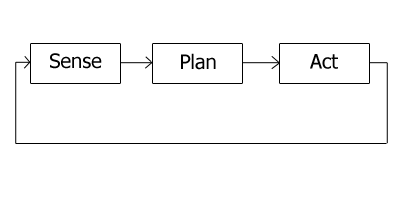
\includegraphics[width=0.4\textwidth]{figure/robotic_paradigm.png}
	\caption{The Sense, Plan, Act robotic paradigm.}
	\label{fig:robotic_paradigm}
\end{figure}

\begin{itemize}
	\item{\textbf{Sense}}: gather information using sensors (camera, IMU, sonar...).
	\item{\textbf{Plan}}:create a world model using all the information, and plan
		the nextmove.
	\item{\textbf{Act}}: carry out the actions that the plan calls for.
\end{itemize}
~\\
This thesis will be focused mainly on the sensing of the drone control, and
more precisely using computer vision algorithms along with machine learning
concepts. However, an important part of the trajectory planning directly
follows the sensing phase, therefore those two first phases of the control loop
can be included in the scope of the project.

To this day, most drones in the robotic research field are running \emph{Robot
Operating System} (ROS) \todo{Add citation}, which is a set of "libraries and
tools to help software developers create robot applications". The implementation
of the computer vision algorithms will be constrained within ROS, and cooperate
with the different control components provided by the project team.\\

\todo{Talk about why CNNs are used more and more in drone racing, and basically
why it is the chosen approach, which leads to tackling the dataset generation
problem.}

As Deep Learning has known an exponential growth during the past decade,
computer vision applications tend to exploit the power of convolutional neural
networks more and more. Thanks to their impressive accuracy in specific problem
solving, CNNs are becoming the main choice for tasks such as: object detection,
object segmentation, object recognition, \emph{etc}\ldots

In drone racing, the latest works, which are often the best performing, tend to
employ CNNs for the sensing part, or even as an all-in-one solution.\\
